
%% ----------------------------------- PREAMBLE ---------------------------------------------- %%

\documentclass[xcolor=dvipsnames, 11pt, table]{beamer}
\let\textmdorig\textmd
\let\textscorig\textsc
\let\textttorig\texttt
%\usecolortheme[named=Black]{structure}
\usetheme[	titleformat frame = smallcaps,
			sectionpage = none,
			numbering = none]{metropolis}
\setbeamertemplate{navigation symbols}{}
\usepackage{beamerfoils}
\usepackage{caption}
\usepackage{tikz}
\usetikzlibrary{arrows,shapes,backgrounds,positioning,patterns,decorations.pathreplacing}
\usepackage{amssymb}
\setbeamertemplate{items}[square]
\usepackage{ragged2e}
\usepackage{etoolbox}
\usepackage{lipsum}
\usepackage{amsmath}
\usepackage{bbm}
%\usepackage{bm}
\usepackage{hyperref}
\usepackage{mathtools}
\usepackage[T1]{fontenc}
\usepackage{lmodern}
\usepackage[sfdefault,scaled=.95]{FiraSans}
%\usepackage{newtxsf}
\usepackage{centernot}

\setbeamertemplate{itemize items}[circle]
\setbeamersize{text margin left = 1em}




%% -------------------------------------- FORMATTING -------------------------------------------- %%

\setbeamercolor{frame}{bg=white}
\setbeamercolor{frametitle}{fg=white,bg=darkgray}
\setbeamercolor{progress bar}{fg=black,bg=gray}
\setbeamercolor{alerted text}{fg=red}
\setbeamercolor{normal text}{fg=black}
\setbeamercolor{progress bar}{fg=black,bg=gray}
\setbeamercolor{title separator}{fg=black,bg=gray}

\setbeamerfont{frametitle}{size=\large,series=\mdseries}
\setbeamerfont{title}{size=\Large,series=\mdseries}
\setbeamerfont{frame}{size=\tiny}

\newcommand{\backupbegin}{
   \newcounter{finalframe}
   \setcounter{finalframe}{\value{framenumber}}
}
\newcommand{\backupend}{
   \setcounter{framenumber}{\value{finalframe}}
}






%% -------------------------------------- TITLE INFO ---------------------------------------------- %%

\title{The Politics of Locating Polling Places  \vspace*{-0.25in}}
\author{	\small Joshua D. Clinton,	\scriptsize{Vanderbilt University}\vspace*{.05in}\\
		\small Nick Eubank,	\scriptsize{Duke University}  \vspace*{.05in}\\
		\small Adriane Fresh,	\scriptsize{Duke University}  \vspace*{.05in}\\
		\small Michael Shepherd,	\scriptsize{Vanderbilt University}
		}
\date{\vspace*{.3in} April 16th, 2021  \vspace*{.125in}}






%% -------------------------------------- BEGIN DOCUMENT ---------------------------------- %%

\begin{document}

\renewcommand<>{\textmd}[1]{%
  \only#2{\textmdorig{#1}}%
}
\renewcommand<>{\textsc}[1]{%
  \only#2{\textscorig{#1}}%
}
\renewcommand<>{\texttt}[1]{%
  \only#2{\textttorig{#1}}%
}



% FRAME: Title Page
% --------------------------

\begin{frame}
	\titlepage
\end{frame}





% FRAME: Motivation
% --------------------------
\begin{frame}[c]{}


	Democratic legitimacy and accountability require that people are freely able to choose their representatives. \\
 
	\pause
	\vspace{0.25in}
	Historically, elites perverted this process for their own political ends. \\  % effectively seek to choose their own electors
	\hspace*{.2in} {\color{gray} \footnotesize e.g. restricting the franchise, gerrymandering}\\ \normalsize
 
 
	\pause
	\vspace{0.25in}
	Less attention given to perversion through the discretion exercised by \alert{local election administrators}. \\
		   \hspace*{.2in} {\color{gray} \footnotesize e.g. polling place locations, voting machine allocations, early voting rules, etc.}\\ \normalsize
 
\end{frame}




% FRAME: Question
% --------------------------
\begin{frame}{Question}

	\pause
	\vspace*{-.18in}
	Do partisan local election administrators in North Carolina systematically move precinct boundaries and polling place locations to manipulate turnout for partisan electoral gain?

	%\pause
	%\vspace*{.2in}
	%Motivations are unknowable \pause $\leadsto$ evidence \alert{consistent} with such a strategy.

\end{frame}





 

\begin{frame}

	\begin{tikzpicture}[remember picture, overlay]

		% Images
		\only<1-4>{\node at (5.8, 0.0)[] {\includegraphics[ width=7.0in,  clip=true,  trim= 0in 0in 0in 0in]{.././Presentation_ExtraFiles/PollingPlace.png}};}

		\only<2->{\node at (6.7, 2.6)[] {\includegraphics[ width=3.5in,  clip=true,  trim= 0in 0in 0in 0in]{.././Presentation_ExtraFiles/News_1.png}};}

		\only<3->{\node at (4.6, 0.5)[] {\includegraphics[ width=3.5in,  clip=true,  trim= 0in 0in 0in 0in]{.././Presentation_ExtraFiles/News_4.png}};}

		\only<4->{\node at (7.85, -2.68)[] {\includegraphics[ width=3.5in,  clip=true,  trim= 0in 0in 0in 0in]{.././Presentation_ExtraFiles/News_5.png}};}

	\end{tikzpicture}

\end{frame}

\begin{frame}{But...}
The plural of anecdote isn't evidence, so we want to be systematic. 
\end{frame}


% FRAME: Our approach
% -------------------

\begin{frame}{Look for evidence of differential targeting of opposition voters}

	\pause
	Collect data on voters, polling places and precincts; 2008, 2012, 2016.

	\pause
	\vspace{0.25in}
	Estimate whether voters of the opposing party (race) to election officials experience differential precinct and polling place changes.

	\pause \footnotesize
	\vspace{0.05in}
	\hspace*{.25in} Changes made in 2012 were made by \color{blue} Democrats.  \color{black}



	\hspace*{.25in} Changes made in 2016 were made by \color{red} Republicans.   \color{black}


	\pause
	\normalsize
	\vspace{0.25in}
	\alert{No evidence} of systematic differential targeting of changes by partisanship or race.



\end{frame}






% FRAME: Local election administration
% ------------------------------------
\begin{frame}{U.S. election administration is decentralized}

	\pause
	States control their own elections.

	\pause
	\vspace*{.25in}
	They typically delegate authority to elected/appointed local entities.  \\
	\hspace*{.2in} {\color{gray} \footnotesize e.g. county boards of election}\\ \normalsize

	\pause
	\vspace*{.25in}
	Implement state and federal law, and exercise their own authority.
	\hspace*{.2in} {\color{gray} \footnotesize e.g. resource allocation, citizen interactions}\\ \normalsize

	\pause
	\vspace*{.25in}
	North Carolina: 3-person appointed county boards, 2 from Governor's party.



\end{frame}






% % FRAME: Discretion
% % -----------------
% \begin{frame}{How might discretion be used}


% \end{frame}





% % FRAME: The history of these things
% % ----------------------------------
% \begin{frame}{The history of these things}


% \end{frame}




% % FRAME: NC
% % ----------------------------------
% \begin{frame}{North Carolina}


% \end{frame}



% %% -------------------------------------- DATA & EMPIRICS ---------------------------------- %%


% \begin{frame}{This Talk}

% \color{gray}
% 1 \hspace*{.25in} Introduction

% \vspace{.1in}
% \color{gray}
% 2 \hspace*{.25in} Framework: Partisan exercise of discretion

% \vspace{.1in}
% \color{black}
% 3 \hspace*{.25in} Empirical Approach: Differential targeting of the opposition

% \vspace{.1in}
% \color{gray}
% 4 \hspace*{.25in} Empirical Approach: Willingness and capacity of counties?

%  \vspace{.1in}
% \color{gray}
% 5 \hspace*{.25in} Conclusion: Why not

% \end{frame}




% FRAME: Broad approach
% -------------------
\begin{frame}{Our empirical approach}

		\pause
		Estimate the \alert{differential} experience of polling place changes by \alert{opposition voters} to the partisan majority of election boards \pause and by \alert{race}.

		\footnotesize \vspace*{.05in}
		$\longrightarrow$ Democrats move the polling places of Republican voters more than Democrat voters \& vice versa.

		\pause
		\vspace{.25in}
		Estimate the differential change in travel time to the polls, conditional on a polling place change.

		\pause
		\vspace{.25in}
		Estimate the differential change in the number of voters per precinct.

\end{frame}

\begin{frame}{Our empirical approach}

	\pause
	Estimate the \alert{differential} experience of polling place changes by \alert{opposition voters} to the partisan majority of election boards. \\
	\pause 
	\begin{itemize}
		\item Precludes us from mis-identifying general partisan trends, like Republicans increasing or decreasing polling places availability everywhere.
	\end{itemize}

	\pause
	Leverage \alert{change} to Democratic control (2004-2008) and subsequent \alert{change} to Republican control (2008-2012)
	\pause 
	\begin{itemize}
		\item Precludes us from mis-identifying general temporal trends, like polling places availability decreasing everywhere.
	\end{itemize}
\end{frame}





% FRAME: North Carolina Context
% -------------------------------------------

\begin{frame}

	\begin{tikzpicture}[remember picture, overlay]

		% Images
		\only<1-2>{\node at (5.8, 0.4)[] {\includegraphics[ width=7.0in,  clip=true,  trim= 0in 0in 0in 0in]{../../50_results_full/Map_Charlotte_Streets.png}};}
		\only<3>{\node at (5.8, 0.41)[] {\includegraphics[ width=7.0in,  clip=true,  trim= 0in 0in 0in 0in]{../../50_results_full/Map_Charlotte_Streets_and_Precincts.png}};}
		\only<4>{\node at (5.8, 0.4)[] {\includegraphics[ width=7.0in,  clip=true,  trim= 0in 0in 0in 0in]{../../50_results_full/Map_Charlotte_Streets_and_Precincts_22_highlighted.png}};}
		\only<5>{\node at (5.8, -1.1)[] {\includegraphics[ width=7.0in,  clip=true,  trim= 0in 0in 0in 0in]{../../50_results_full/Map_Charlotte_Precinct_22_highlighted.png}};}
		\only<6>{\node at (5.8, -1.1)[] {\includegraphics[ width=7.0in,  clip=true,  trim= 0in 0in 0in 0in]{../../50_results_full/Map_Charlotte_Precinct_22_highlighted_race_shaded.png}};}
		\only<7>{\node at (5.8, -1.1)[] {\includegraphics[ width=7.0in,  clip=true,  trim= 0in 0in 0in 0in]{../../50_results_full/Map_Charlotte_Precinct_22_2008.png}};}
		\only<8>{\node at (5.8, -1.1)[] {\includegraphics[ width=7.0in,  clip=true,  trim= 0in 0in 0in 0in]{../../50_results_full/Map_Charlotte_Precinct_22_2012.png}};}
		\only<9>{\node at (5.8, -1.1)[] {\includegraphics[ width=7.0in,  clip=true,  trim= 0in 0in 0in 0in]{../../50_results_full/Map_Charlotte_Precinct_22_2016.png}};}


		% % Text
		% \only<2-4>{\node[anchor=north east] at (8.0, 1.2) {\scriptsize \textsc{Central business district}};}
		% \only<1-8>{\node[text=white,fill=black, anchor=north east] at (12.2, 4.0) {\textsc{Charlotte, Mecklenburg County, North Carolina}};}
		% \only<4-8>{\node[text=white,fill=black, anchor=north east] at (12.2, 3.45) {\textsc{Electoral precinct \#22}};}

		% \only<7->{\node[anchor=north west,text=black] at (5.7, -0.00) {\scriptsize \textsc{2008 polling}};}
		% \only<7->{\node[anchor=north west,text=black] at (5.7, -0.30) {\scriptsize \textsc{place location}};}


		% \only<8->{\node[anchor=north west,text=blue] at (4.7, -2.0) {\scriptsize \textsc{2012 polling}};}
		% \only<8->{\node[anchor=north west,text=blue] at (4.7, -2.3) {\scriptsize \textsc{place location}};}

		% \only<9->{\node[anchor=north west,text=red] at (6.0, 2.2) {\scriptsize \textsc{2016 polling}};}
		% \only<9->{\node[anchor=north west,text=red] at (6.0, 1.9) {\scriptsize \textsc{place location}};}

		% \only<6->{\node[anchor=north west,text=black] at (-0.25, -4.6) {\tiny Darker shading is higher \% of census block black.};}

	\end{tikzpicture}


\end{frame}




% FRAME: Data
% -------------------
\begin{frame}{We assemble an individual-level dataset}

	\pause
	Collect panel data on every registered voter in North Carolina, 2008-2016. \vspace*{-.08in} \\
	{\color{gray}\tiny{(North Carolina State Board of Election (NCSBE))}} \color{black} \normalsize \\

	\footnotesize \vspace*{.05in}
		\hspace*{.2in} $>8$ million individuals ($>5$ million eligible voters in both 2008 \& 2012) \\
		\hspace*{.2in} Restrict the sample to voters who have not moved. \\
	% previous studies have examined just a few precincts at any one time



	\pause \normalsize \vspace{0.15in}
	Collect data on all precinct boundaries and polling place locations. \vspace*{-.08in} \\
	{\color{gray}\tiny{(NC Democratic Party; County boards of election (various); NCSBE)}} \color{black} \normalsize \\


	\pause \normalsize
	\vspace{.15in}
	Geolocate voter residences, match to precincts \& polling places.  \vspace*{-.08in} \\
	%{\color{gray}\tiny{(Google maps API)}} \color{black} \normalsize \\


\end{frame}





% % FRAME: Approach
% % -------------------------

% \begin{frame}{}


% 	Simple difference in means

% \end{frame}




% % FRAME: Approach
% % -------------------------

% \begin{frame}{Estimating differential targeting by partisanship}

% 	\pause
% 	For individual $i$, in county $c$, in election year $t$, we estimate \footnotesize

% 	\vspace*{-.1in}
% 	\begin{eqnarray*}
% 		Pr(\Delta Y_{i,c,t}) = \alpha_{c} + \gamma_{t} + \alpha_{c}\times\gamma_{t} + \beta_1 Opposition_{i,t} + \beta_2 Independent_{i,t} \nonumber \\
% 	  + \beta_{4}Age_{i,t} + \beta_{5}Age_{i,t}^{2} + \epsilon_{i,t} \nonumber
% 	\end{eqnarray*}

% 	\pause
% 	\vspace{.1in}
% 	\hspace*{0.75in} $Y_{i,c,t}$ 									\hspace*{.4in} polling place; voters-per-precinct \\
% 	\hspace*{0.85in} $\alpha_{c}$ 								\hspace*{.4in} county FE \\
% 	\hspace*{0.891in} $\gamma_{t}$ 								\hspace*{.4in} election year FE \\
% 	\hspace*{0.3in} $Opposition_{i,t}$ 								\hspace*{.4in} =1 if opposition party to governor \\
% 	\hspace*{0.7in} $Age_{i,t}$ 											\hspace*{.4in} voter age \\


% 	\pause
% 	\vspace{.3in} \normalsize
% 	Also estimate cross-sectional specifications for \color{blue}{2012} \color{black} and \color{red}{2016}. \\



% \end{frame}





% % FRAME: Approach
% % -------------------------

% \begin{frame}{And examine whether there is an additional effect of race}

% 	For individual $i$, in county $c$, in election year $t$, we estimate \footnotesize

% 	\vspace*{-.1in}
% 	\begin{eqnarray*}
% 	Pr(\Delta Y_{i,c,t}) = \alpha_{c} + \gamma_{t} + \alpha_{c}\times\gamma_{t} + \beta_1 WhiteOpposition_{i,t}   \nonumber \\
% 	 + \beta_2 BlackOpposition_{i,t} + \beta_3 OtherOpposition_{i,t} + \beta_4 WhiteUnaffiliated_{i,t}  \nonumber \\
% 	 + \beta_5 OtherUnaffiliated + \beta_{4}Age_{i,t} + \beta_{5}Age_{i,t}^{2}  + \epsilon_{i,t}.
% 	\end{eqnarray*}

% \end{frame}












% FRAME: Polling Place Changes Panel Results
% -------------------------------------

\begin{frame}{}
	\begin{figure}[htbp]
		\centering
		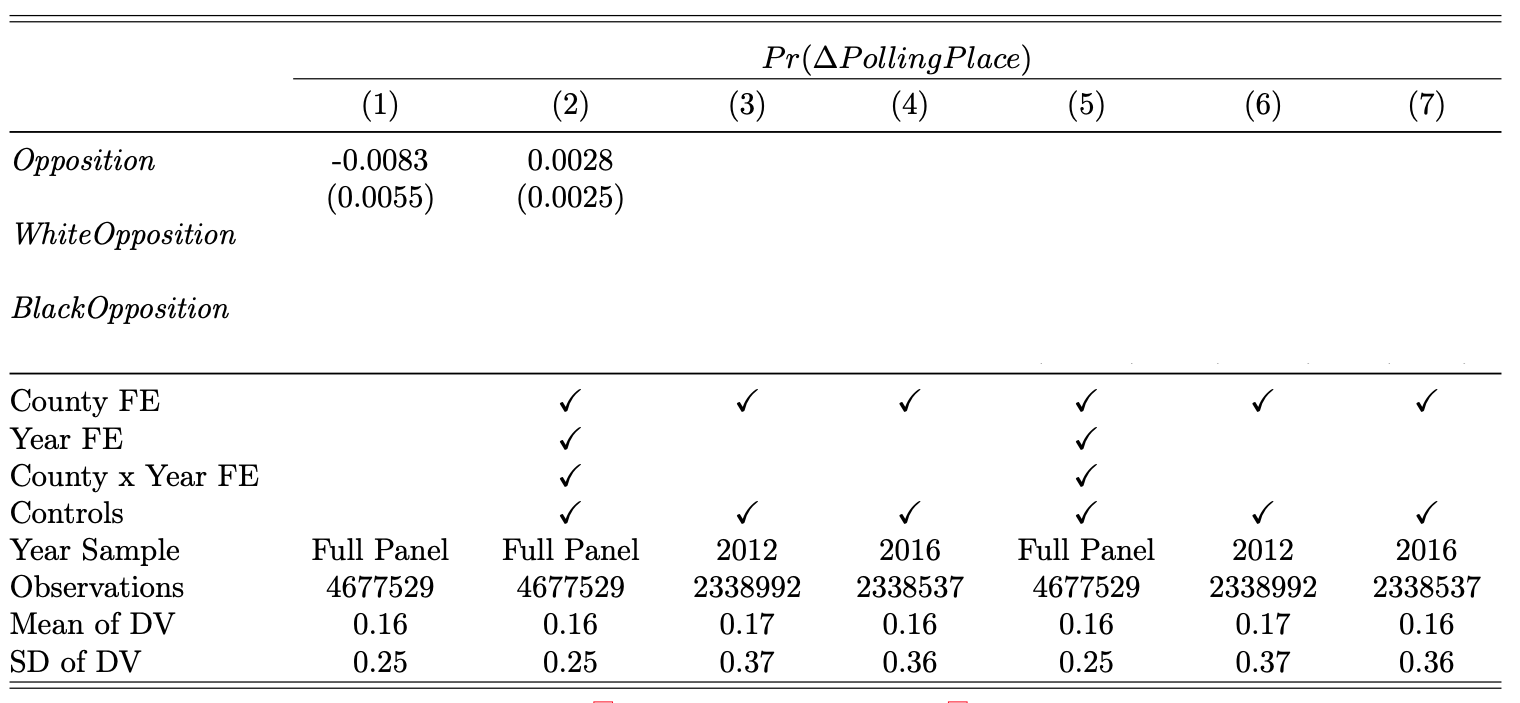
\includegraphics[ width=\textwidth]{ppchange_1.png}
	\end{figure}
\end{frame}

\begin{frame}{}
	\begin{figure}[htbp]
		\centering
		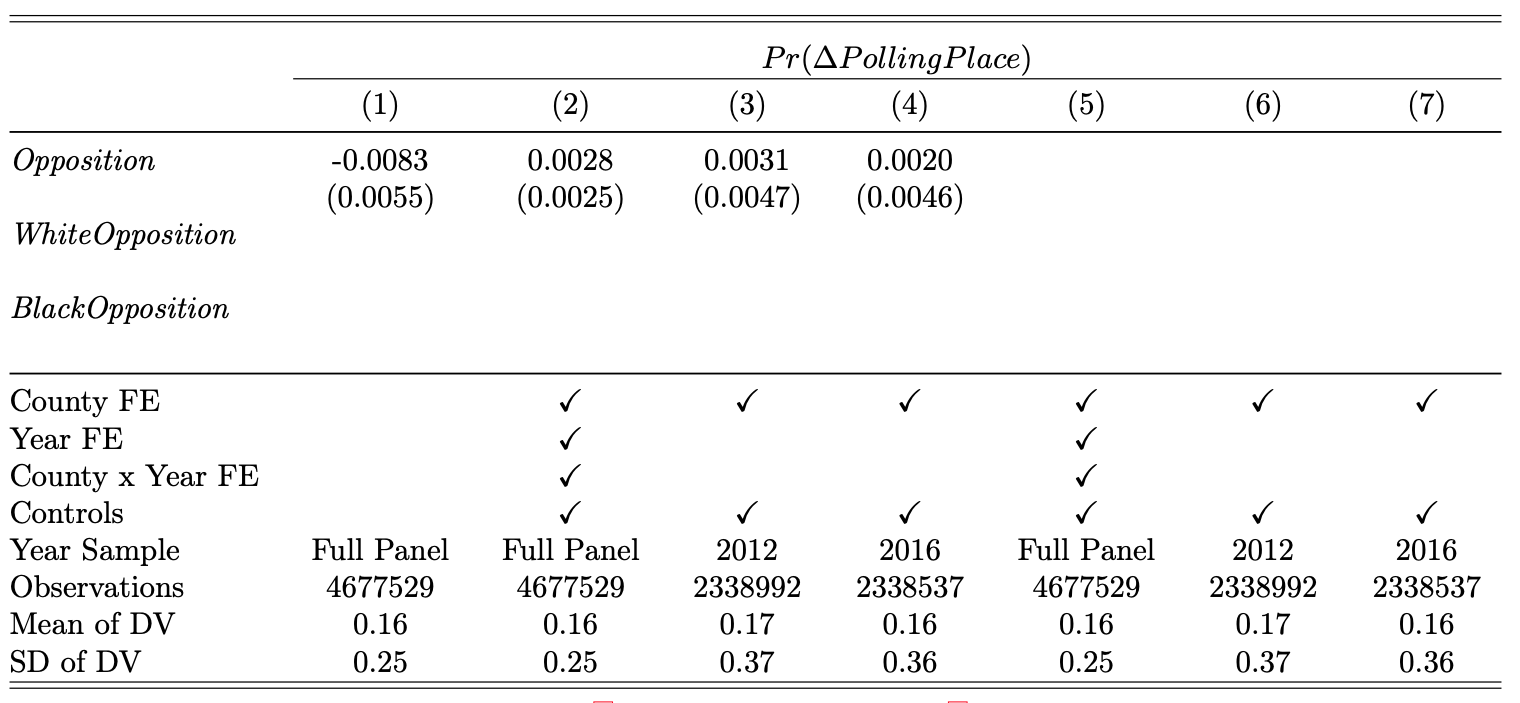
\includegraphics[ width=\textwidth]{ppchange_2.png}
	\end{figure}
\end{frame}

\begin{frame}{}
	\begin{figure}[htbp]
		\centering
		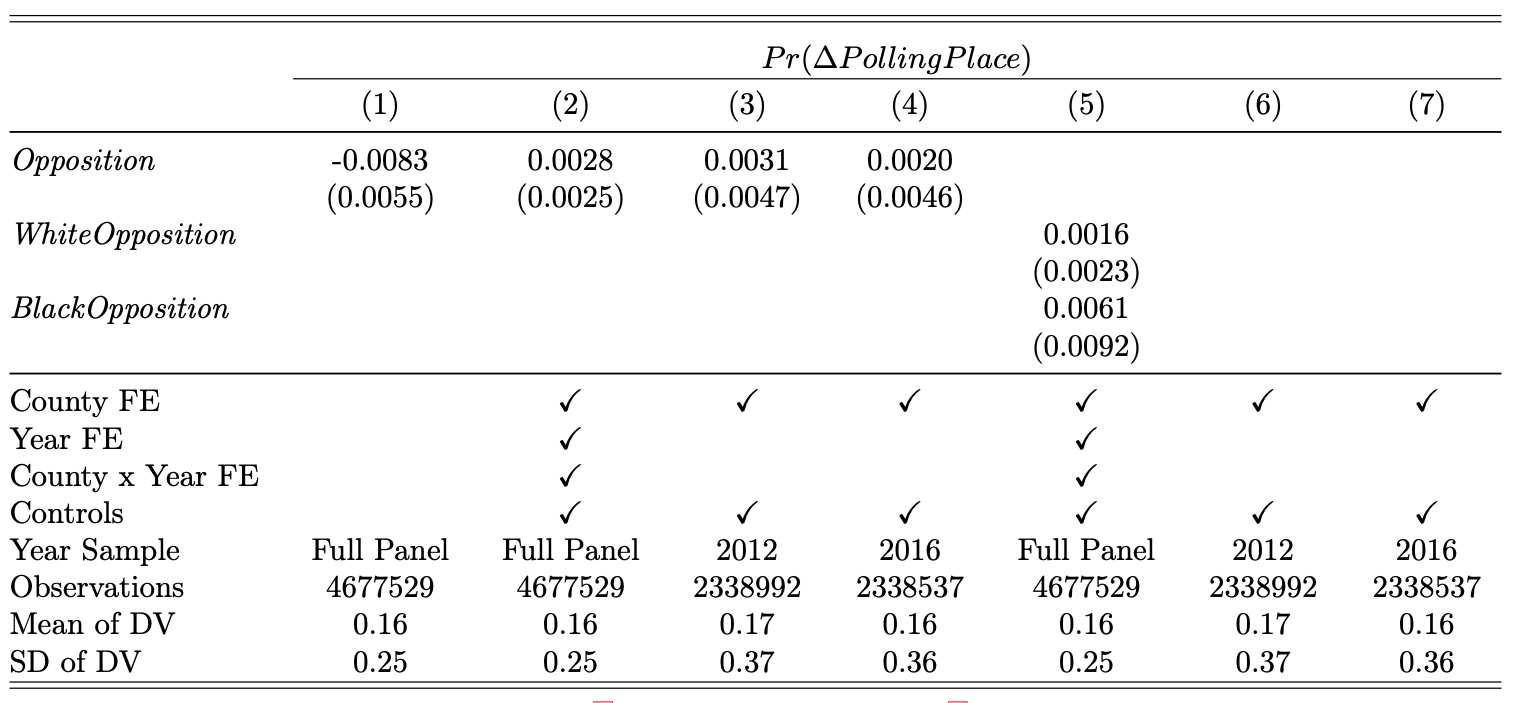
\includegraphics[ width=\textwidth]{ppchange_3.jpg}
	\end{figure}
\end{frame}

\begin{frame}{}
	\begin{figure}[htbp]
		\centering
		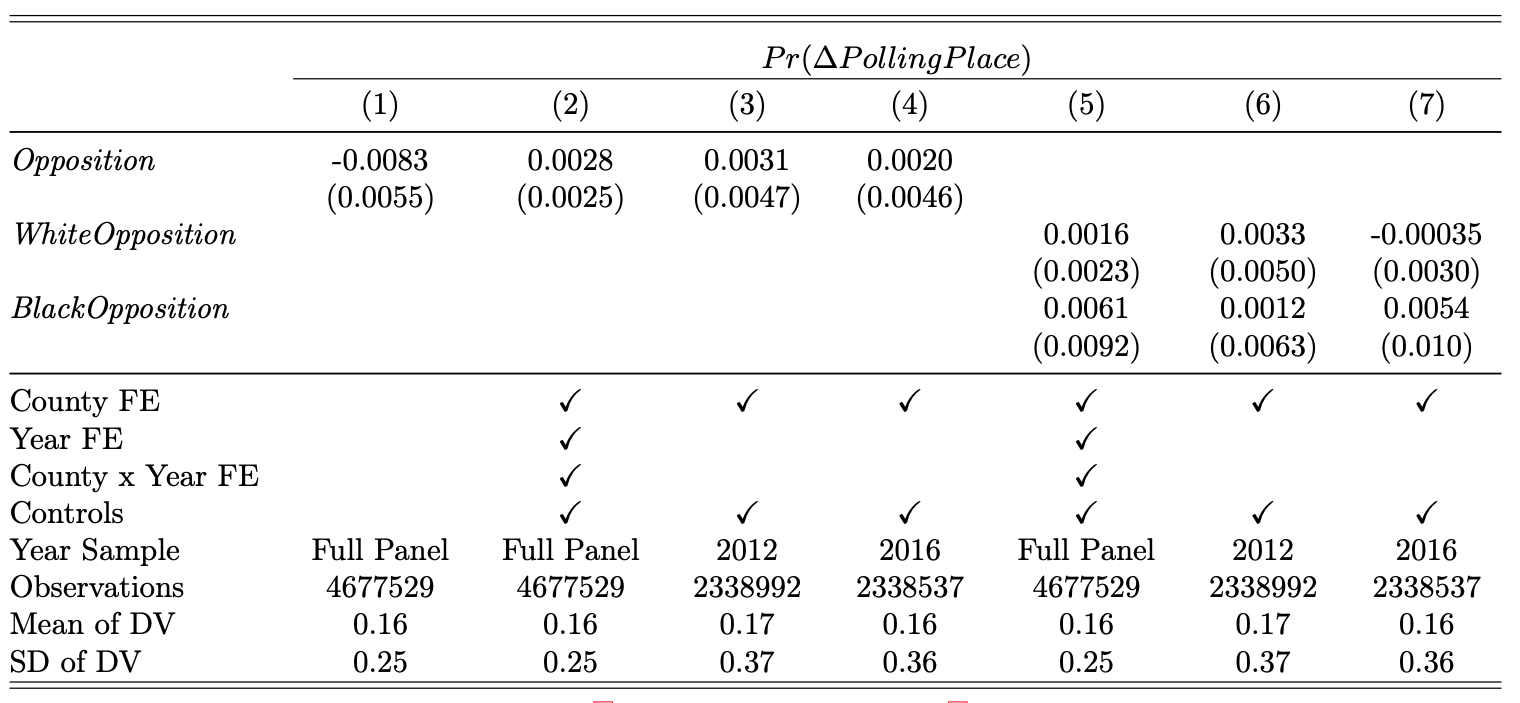
\includegraphics[ width=\textwidth]{ppchange_full.png}
	\end{figure}
\end{frame}




\begin{frame}{}
	\begin{figure}[htbp]
		\centering
		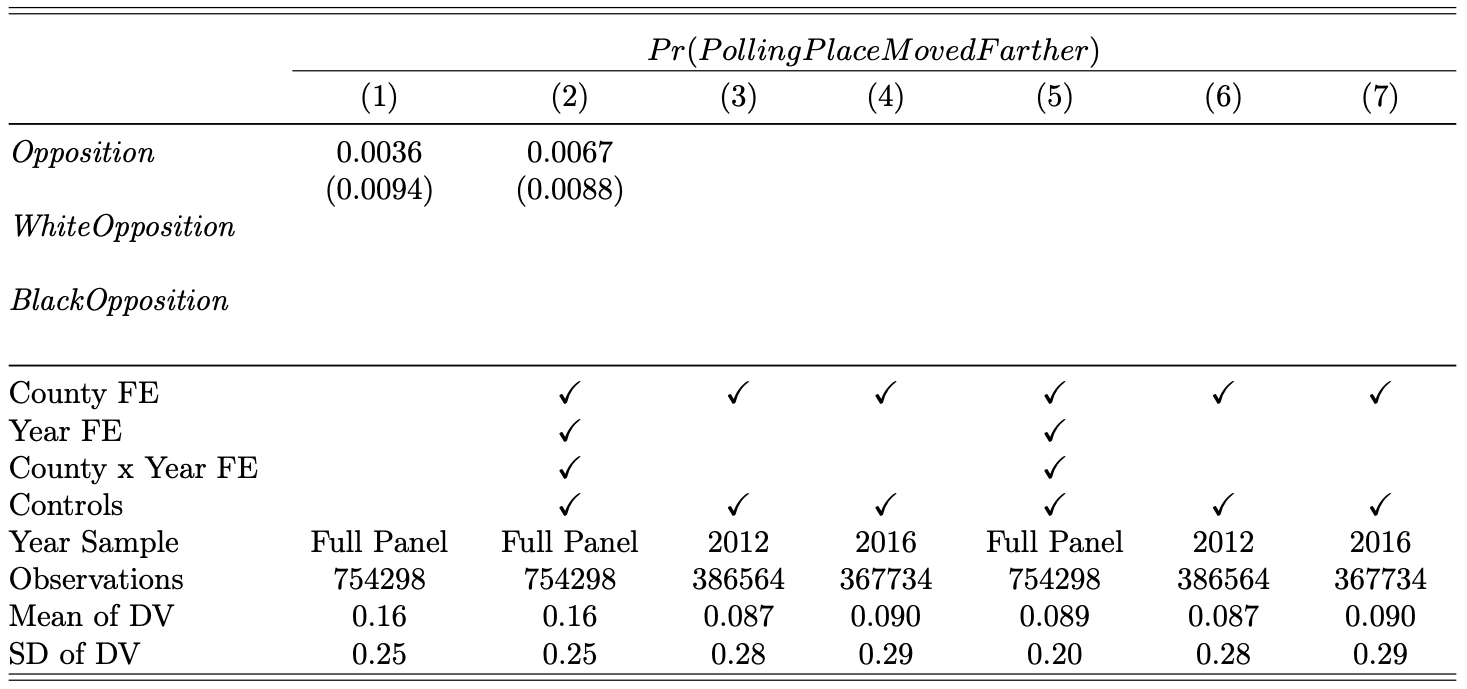
\includegraphics[ width=\textwidth]{ppmove_1.png}
	\end{figure}
\end{frame}

\begin{frame}{}
	\begin{figure}[htbp]
		\centering
		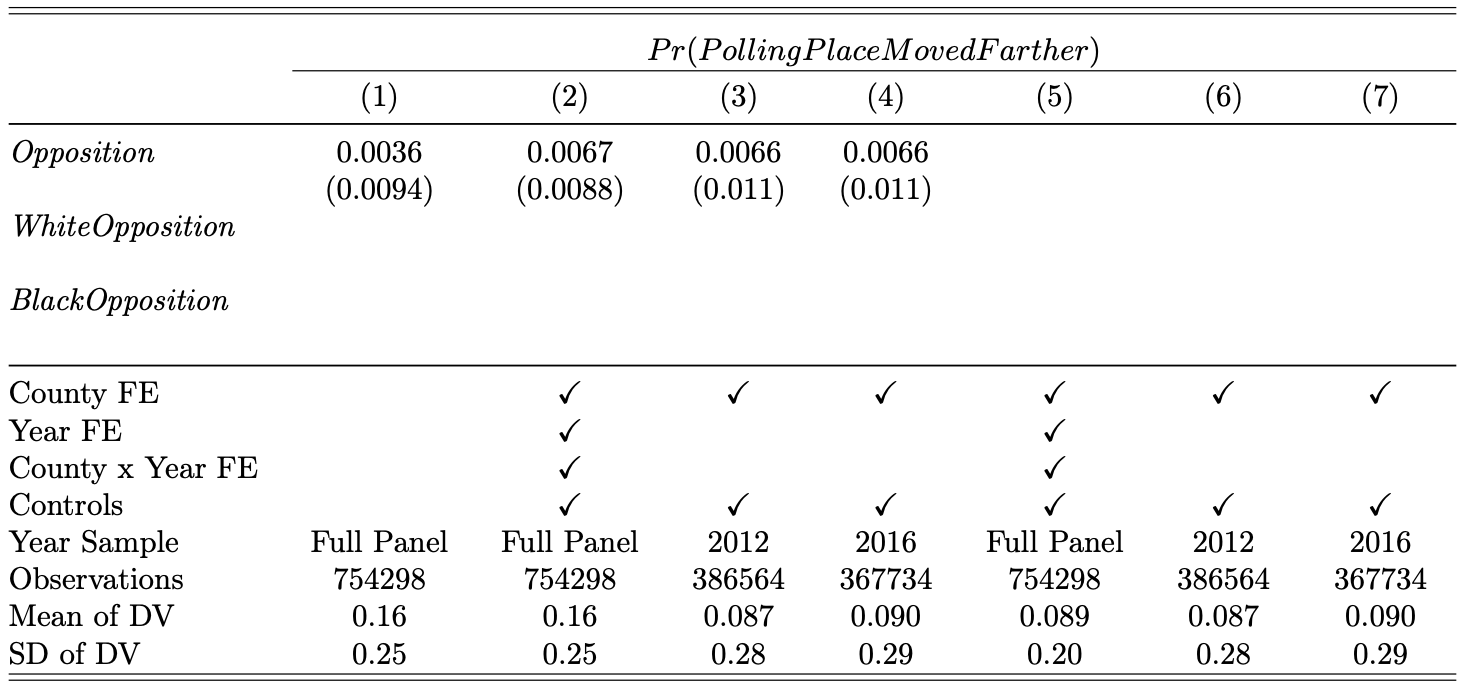
\includegraphics[ width=\textwidth]{ppmove_2.png}
	\end{figure}
\end{frame}


\begin{frame}{}
	\begin{figure}[htbp]
		\centering
		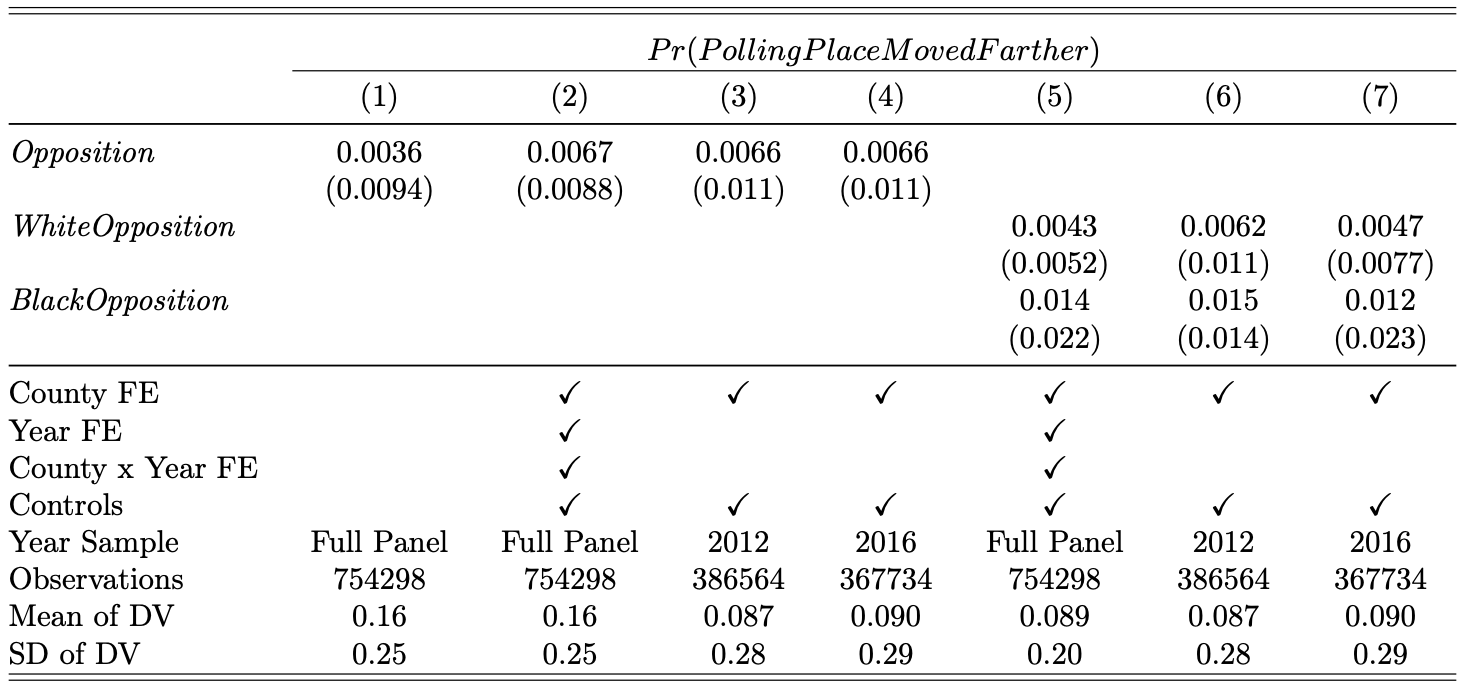
\includegraphics[ width=\textwidth]{ppmove_full.png}
	\end{figure}
\end{frame}





\begin{frame}

	\begin{tikzpicture}[remember picture, overlay]

		% Images
		\node at (5.8, 0.0)[] {\includegraphics[ width=7.0in,  clip=true,  trim= 0in 0in 0in 0in]{.././Presentation_ExtraFiles/PollingPlace.png}};

		\node at (6.7, 2.6)[] {\includegraphics[ width=3.5in,  clip=true,  trim= 0in 0in 0in 0in]{.././Presentation_ExtraFiles/News_1.png}};

		\node at (4.6, 0.5)[] {\includegraphics[ width=3.5in,  clip=true,  trim= 0in 0in 0in 0in]{.././Presentation_ExtraFiles/News_4.png}};

		\node at (7.85, -2.68)[] {\includegraphics[ width=3.5in,  clip=true,  trim= 0in 0in 0in 0in]{.././Presentation_ExtraFiles/News_5.png}};

	\end{tikzpicture}

\end{frame}

\begin{frame}{What's Going On?}
We think polling places regularly have to be moved, and so some of those moves will necessarily advantage party in power. \\
\pause But others will \emph{dis}advantage party in power. \\
\vspace{0.15cm}
We think there's a selection effect in reporting.  
\end{frame}

\begin{frame}{}
	\begin{tikzpicture}[remember picture, overlay]

			\node at (6.0, -0.52)[] {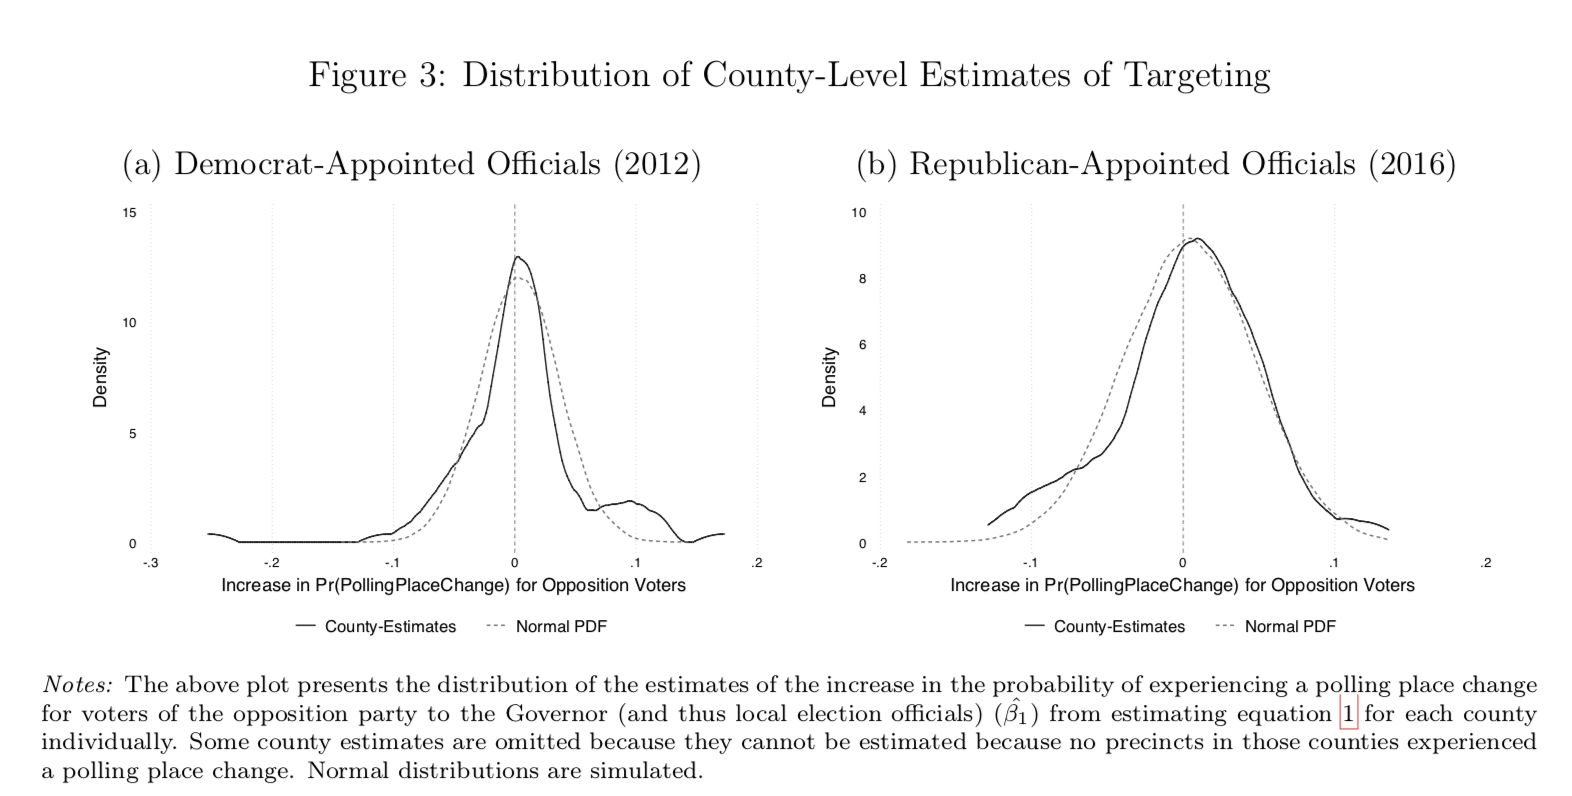
\includegraphics[ width=5.00in,  clip=true,  trim= 0in 0in 0in 0in]{Fig4.png}};

	\end{tikzpicture}


\end{frame}

\begin{frame}{}
	\begin{figure}[htbp]
		\centering
		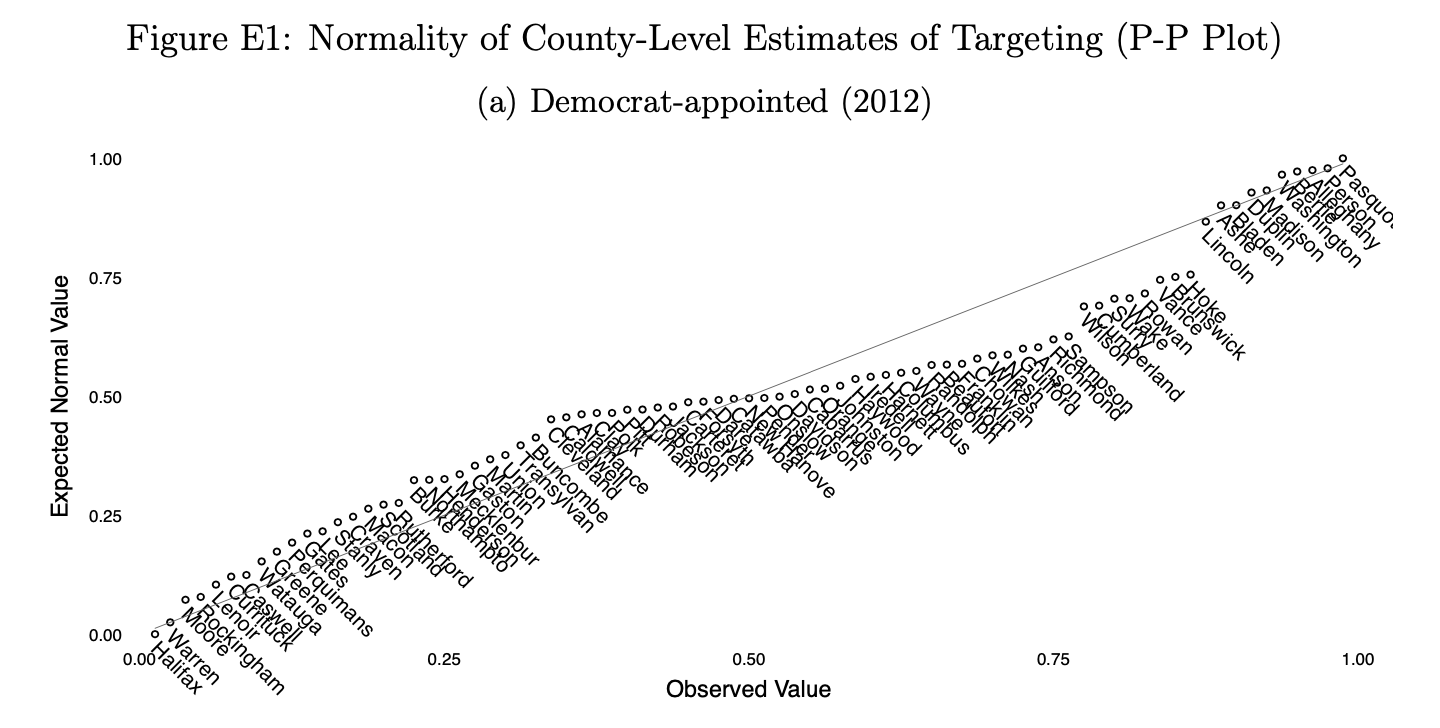
\includegraphics[ width=\textwidth]{normality_1.png}
	\end{figure}
\end{frame}

\begin{frame}{}
	\begin{figure}[htbp]
		\centering
		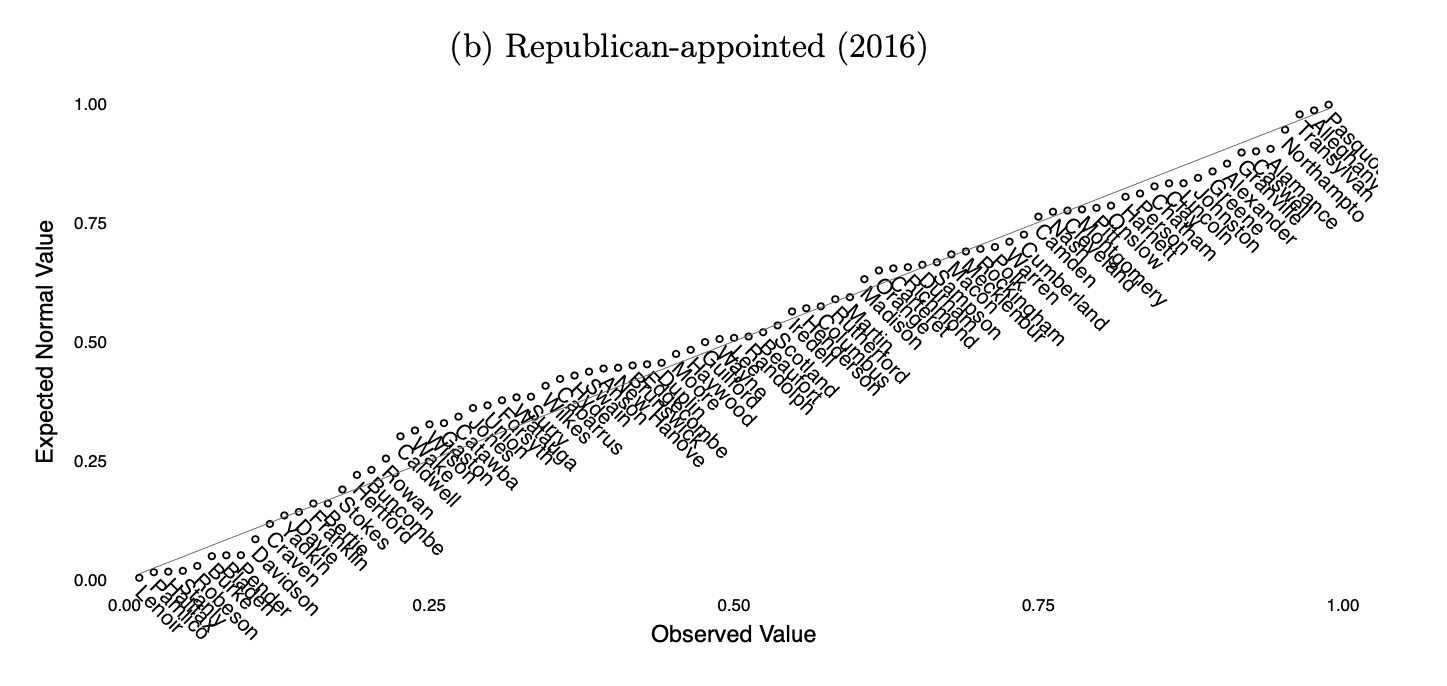
\includegraphics[ width=\textwidth]{normality_2.png}
	\end{figure}
\end{frame}



% FRAME: Substitution
% ----------------------------

% \begin{frame}{}

% 	\begin{tikzpicture}[remember picture, overlay]

% 			\only<1-2>{\node at (3.25, 1.25)[] {\includegraphics[ width=2.75in,  clip=true,  trim= 0in 0in 0in 0in]{../Presentation_ExtraFiles/NC_VRA_1a.png}};}

% 			\only<1-2>{\node at (3.25, -2.25)[] {\includegraphics[ width=2.75in,  clip=true,  trim= 0in 0in 0in 0.25in]{../Presentation_ExtraFiles/NC_VRA_1b.png}};}

% 			\only<1-2>{\node at (4.0, -4.25)[] {\includegraphics[ width=1.5in,  clip=true,  trim= 0in 0in 0in 0.296in]{../Presentation_ExtraFiles/NC_VRA_1c.png}};}


% 			\only<2->{\node[] at (9.0, 4.0) {\footnotesize U.S. Civil Rights Commission:};}

% 			\only<2->{\node[] at (9.0, 2.0) {\scriptsize \texttt{``the Polling Place for South Smiths }};}
% 			\only<2->{\node[] at (9.0, 1.6) {\scriptsize \texttt{would be eliminated ''}};}


% 	\end{tikzpicture}


% \end{frame}






% %% -------------------------------------- CONCLUSION ---------------------------------- %%




% FRAME: Implications
% ------------------------

\begin{frame}{Implications }


	\pause \vspace{.25in}
	Despite claims to the contrary, we find no evidence of systematic manipulation of precincts and polling places in North Carolina.


	\pause
	\vspace{0.15in}

	Illustrates importance of \alert{systematic} evaluation of claims of manipulation.\\
	\pause For journalists \emph{and} voting rights advocates.

	\pause
	\vspace{0.15in}

	This is specific to North Carolina, and the period being studied.


\end{frame}






% % FRAME:  End Frame Plain
% % ------------------------------------


% \begin{frame}[plain]


% \end{frame}








%% ---------------------------------------------------------------- END DOCUMENT ---------------------------------------------------------------- %%

\end{document}
